\newpage
\setcounter{subsection}{0}
\section{CONTEXTO DEL PROYECTO}

\subsection{Blockchain, contratos inteligentes y stablecoins}

Una cadena de bloques es una estructura de datos distribuida, cronológica y enlazada criptográficamente, en
la que 
un conjunto de nodos independientes mantiene una réplica del registro y aplica un protocolo de consenso para
acordar 
el orden y la validez de las transacciones sin requerir una autoridad central. Para evitar ataques de
denegación de 
servicio y de doble gasto, las blockchains públicas tradicionales se apoyan en dos paradigmas principales de
consenso:

\begin{itemize}
    \item \textbf{Proof of Work (PoW):} Introducido por Bitcoin \cite{nakamoto2008bitcoin}, requiere que los
nodos 
    validadores (mineros) resuelvan complejos acertijos criptográficos utilizando potencia de cómputo. El
primero 
    en resolver el acertijo tiene el derecho de proponer el siguiente bloque, asegurando la red a través del
gasto intensivo de energía.

    \item \textbf{Proof of Stake (PoS):} Alternativa que reemplaza el consumo energético por el compromiso
financiero. 
    Los validadores bloquean una cantidad de criptomonedas nativas (colateral) en la red para tener la
probabilidad de proponer 
    nuevos bloques, penalizando económicamente los comportamientos maliciosos.
\end{itemize}

Sobre esta infraestructura descentralizada, los contratos inteligentes son programas informáticos con estado
persistente 
y ejecución determinística cuyas transiciones se ejecutan bajo el mismo conjunto de reglas en cada nodo. En
el ámbito del 
ticketing, el contrato inteligente actúa como una bóveda lógica auto-ejutable que regula la propiedad,
transfiere el activo 
y distribuye las regalías al organizador de forma automática al recibir el pago.

Sin embargo, las criptomonedas nativas presentan una volatilidad de precio que introduce fricción comercial
en el e-commerce 
cotidiano. Para mitigar esta problemática, el ecosistema blockchain introdujo las \textit{Stablecoins}
(monedas estables), 
tokens criptográficos cuyo valor se encuentra anclado en paridad $1:1$ a una moneda fiduciaria de curso legal 
(como el dólar estadounidense). En este trabajo se adopta USDC (USD Coin) como token de pago, un criptoactivo
respaldado 
en su totalidad por reservas de efectivo y bonos del Tesoro de EE. UU. \cite{sdf2024stablecoins}, lo que
permite que el comprador 
de un boleto pague una tarifa fija en dinero estable mientras disfruta de la programabilidad y liquidación
atómica on-chain.

\subsection{Red Stellar y protocolo de consenso (SCP)}

Stellar es una blockchain pública orientada a la transferencia rápida de valor digital y a la emisión de
activos tokenizados. 
A diferencia de las redes tradicionales basadas en PoW o PoS, la red Stellar opera bajo el \textit{Stellar
Consensus Protocol} 
(SCP), una implementación del modelo de Acuerdo Bizantino Federado (FBA, \textit{Federated Byzantine
Agreement}) 
\cite{mazieres2015stellar}. El FBA establece un paradigma descentralizado en el cual los participantes del
sistema no son 
preseleccionados por una autoridad central, sino que cada nodo declara individualmente sus propios círculos
de confianza 
denominados \textbf{rebanadas de quórum} (Quorum Slices).

Un quórum global en SCP se define como un conjunto de nodos que contiene al menos una rebanada de quórum para
cada uno de sus 
miembros. Para ilustrar este concepto, la documentación oficial de Stellar propone un modelo de toma de
decisiones locales 
mediante un ejemplo compuesto por cuatro participantes: Bob, Cal, Cam y Deb. En este escenario, Bob desea
acordar el estado 
de una transacción y define sus condiciones de confianza de la siguiente manera:

\begin{enumerate}
    \item Confía de forma conjunta en la opinión de Cal y Cam.
    \item Confía de forma independiente en la opinión de Deb.
\end{enumerate}

Esto significa que Bob posee dos rebanadas de quórum válidas: el conjunto $\{\text{Bob}, \text{Cal},
\text{Cam}\}$ y el conjunto 
$\{\text{Bob}, \text{Deb}\}$. Para que Bob valide un bloque, es necesario que él y todos los miembros de al
menos una de sus 
rebanadas estén de acuerdo. Este flujo de confianza subjetiva y local se representa gráficamente en la
Figura~\ref{fig:cal_cam_bob_deb}.

\begin{figure}[H]
    \centering
    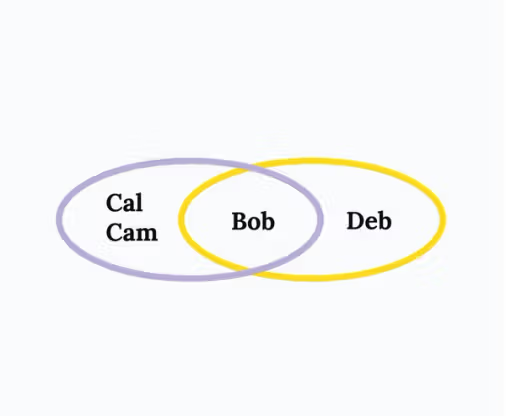
\includegraphics[width=0.55\textwidth]{Imagenes/conjunto_cal_cam_deb.png}
    \caption{Ejemplo de rebanadas de quórum (Quorum Slices) para el nodo Bob.}
    \label{fig:cal_cam_bob_deb}
\end{figure}

El SCP garantiza que, a través de la superposición de estas rebanadas de confianza locales entre múltiples
participantes en 
la red, se formen quórums globales interconectados. La propiedad fundamental del SCP es la
\textbf{intersección de quórums}: 
si todo par de quórums de la red comparte al menos un nodo correcto (no defectuoso ni malicioso), el sistema
mantendrá seguridad 
absoluta (\textit{safety}) impidiendo la bifurcación del registro histórico (doble gasto), incluso en
presencia de nodos bizantinos. 
El SCP prioriza en todo momento la consistencia del registro sobre la disponibilidad temporal
(\textit{liveness}), deteniendo la 
red en caso de que no exista consenso en lugar de escribir transacciones inconsistentes. En la
Figura~\ref{fig:consenso_scp} se 
muestra la representación matemática del solapamiento de estas rebanadas y nodos.

\begin{figure}[H]
    \centering
    \begin{subfigure}[b]{0.35\textwidth}
        \centering
        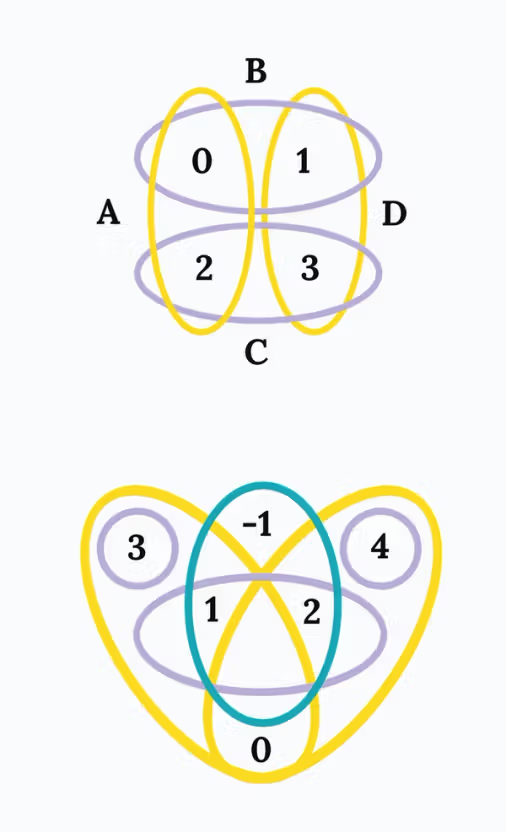
\includegraphics[width=\textwidth]{Imagenes/conjunto_matematico.png}
        \caption{Intersección de quórums lógicos.}
        \label{fig:conjunto_matematico}
    \end{subfigure}

    \bigskip

    \begin{subfigure}[b]{0.95\textwidth}
        \centering
        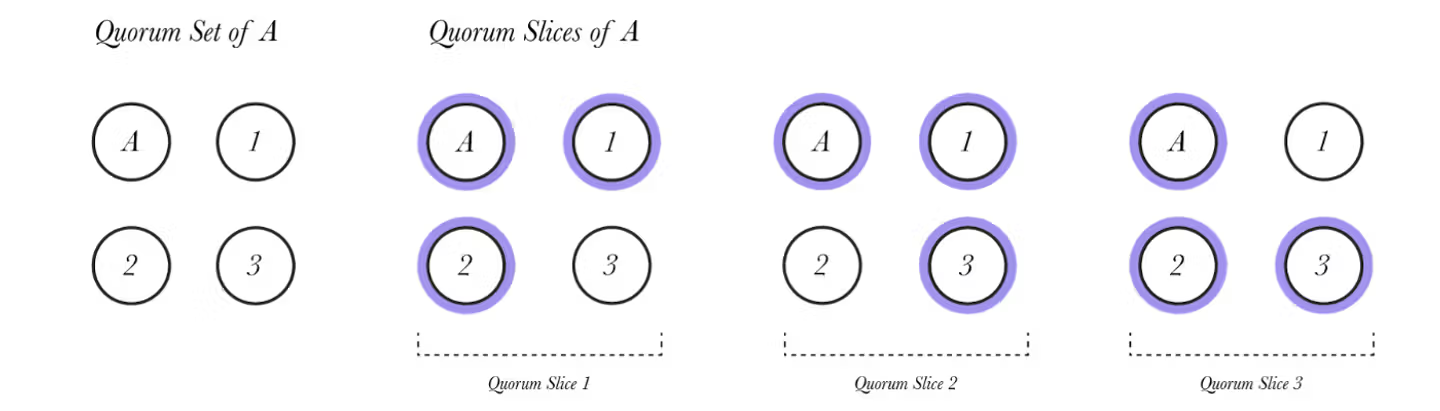
\includegraphics[width=\textwidth]{Imagenes/quorum.png}
        \caption{Configuración de consenso entre nodos.}
        \label{fig:quorum_nodos}
    \end{subfigure}
    \caption{Representación matemática e intersección de quórums en el protocolo SCP.}
    \label{fig:consenso_scp}
\end{figure}

\subsection{Sostenibilidad y consumo de recursos en perspectiva industrial}

La adopción de tecnologías descentralizadas se enfrenta de manera recurrente a debates de carácter ecológico.
La minería 
clásica de Bitcoin (PoW) consume aproximadamente $150$\,TWh de energía eléctrica al año
\cite{cbeci2024bitcoin}, una huella 
energética equiparable al consumo anual de países enteros como Argentina o Ucrania, lo cual se traduce en una
emisión 
significativa de gases de efecto invernadero si la matriz energética depende de combustibles fósiles.

En contraste, el mecanismo SCP de Stellar no involucra minería por cómputo intensivo ni colateralización
forzosa de validadores, 
limitándose al intercambio asíncrono de mensajes firmados criptográficamente. Una evaluación del impacto
ecológico comisionada 
por la Stellar Development Foundation en conjunto con la consultora PwC US bajo el Marco de Evaluación de
Sostenibilidad de 
Blockchain (BSF, \textit{Blockchain Sustainability Framework}) determinó los siguientes valores operativos
para la red 
\cite{sdf2024sustainability}:

\begin{itemize}
    \item \textbf{Consumo de energía por transacción:} Aproximadamente $0{,}173$\,Wh (equivalente a
$0{,}000173$\,kWh).
    \item \textbf{Emisión de carbono por transacción:} Aproximadamente $0{,}062$ gramos de $CO_2$ equivalente
($g\,CO_2e$).
    \item \textbf{Consumo total del ecosistema:} La energía eléctrica anual total requerida por el conjunto
completo de validadores activos de Stellar equivale al consumo energético de un único servidor web
convencional de gama media.
\end{itemize}

Para poner estas cifras en perspectiva dentro de la infraestructura tecnológica y económica moderna, la
Tabla~\ref{tab:sostenibilidad} 
contrasta el consumo de energía unitario estimado de diferentes actividades y sectores contra el
procesamiento de una transacción 
en Stellar.

\begin{table}[H]
\centering
\small
\renewcommand{\arraystretch}{1.3}
\definecolor{rowgray}{gray}{0.96}
\caption{Comparativa de consumo energético estimado por operación/unidad.}
\label{tab:sostenibilidad}
\begin{tabularx}{\textwidth}{>{\raggedright\arraybackslash}p{6.0cm} >{\raggedright\arraybackslash}p{3.5cm}
>{\raggedright\arraybackslash}X}
\toprule
\rowcolor{rowgray}
\textbf{Actividad / Sector} & \textbf{Consumo de energía} & \textbf{Equivalencia en transacciones Stellar} \\
\midrule
Transacción en Stellar (SCP) & $0{,}173$\,Wh ($0{,}000173$\,kWh) & $1$ \\
\rowcolor{rowgray}
Consulta simple en buscador tradicional & $\approx$\,0{,}30\,Wh & $\approx$\,1{,}7 \\
Consulta simple a modelo de IA (LLM) & $\approx$\,3{,}00--9{,}00\,Wh & $\approx$\,17--52
\cite{iea2024electricity} \\
\rowcolor{rowgray}
Transacción clásica de tarjeta de crédito & $\approx$\,1{,}50--2{,}50\,Wh & $\approx$\,8--14 \\
Producción de $1$\,kg de cemento (Construcción) & $\approx$\,1\,300--1\,500\,Wh & $\approx$\,7\,500--8\,600 \\
\rowcolor{rowgray}
Transacción promedio de Bitcoin (PoW) & $\approx$\,800--1\,200\,kWh &
$\approx$\,4\,600\,millones--6\,900\,millones \cite{cbeci2024bitcoin} \\
\bottomrule
\end{tabularx}
\end{table}

A nivel global, mientras que los centros de datos (impulsados en gran parte por el crecimiento exponencial
del entrenamiento 
e inferencia de modelos de inteligencia artificial y la computación en la nube) proyectan consumir más de
$1\,000$\,TWh para 
el año 2026 \cite{iea2024electricity} y el sector de la construcción tradicional aporta cerca del 37\,\% de las emisiones de 
carbono mundiales, la red Stellar se establece como una de las infraestructuras de liquidación financiera más
sostenibles de 
la actualidad. La integración de este middleware Web2.5 no penaliza la huella de carbono de los eventos
masivos, sino que la 
optimiza en comparación con el despliegue de contratos inteligentes sobre cadenas heredadas basadas en PoW o
redes centralizadas 
de alta fricción física (transporte y tickets en papel).

\subsection{Soroban, NFTs y tokens de pago}

Soroban es la plataforma de contratos inteligentes de Stellar. Los contratos se escriben en Rust contra el
crate \texttt{soroban-sdk} (versión 23 en este trabajo) y se compilan al target \texttt{wasm32v1-none}. El
modelo de ejecución es determinístico, sin acceso a fuentes no reproducibles (relojes locales, aleatoriedad
no derivada del ledger, llamadas al sistema operativo).

Soroban gestiona tres tipos de almacenamiento: \texttt{Persistent}, \texttt{Temporary} e \texttt{Instance},
cada uno con un costo de \textit{rent} distinto. La emisión de eventos se realiza mediante
\texttt{events().publish()}: cada evento contiene \textit{topics} indexables y un \textit{body} serializable,
y se almacena en el meta del ledger, lo que permite a los indexadores externos consumirlo sin afectar el
costo de \textit{rent} del contrato.

El estándar NFT en Soroban define una representación de activos no fungibles con identificador único,
propietario tipo \texttt{Address} y reglas de transferencia controladas por el contrato emisor. En este
trabajo se extiende este estándar con un esquema de versionado: cada boleto se identifica por la tupla
(\texttt{ticket\_root\_id}, \texttt{version}), donde \texttt{version} se incrementa en cada operación de
reventa mediante un patrón \textit{burn/remint}.

El activo nativo de la red, XLM, y cualquier activo emitido en Stellar se exponen como tokens compatibles con
la interfaz estándar de Soroban a través del \textit{Stellar Asset Contract} (SAC). Esto permite que las
operaciones de pago de la compra de reventa se ejecuten dentro del mismo flujo de invocación del contrato del
evento, sin transacciones separadas para el pago y la transferencia de propiedad.

\subsection{Análisis del Contexto}

El análisis comparativo de soluciones del mercado y de la literatura técnica permite identificar tres
categorías de antecedentes: (i) plataformas tradicionales de reventa basadas en QR estáticos y conciliación
bancaria; (ii) soluciones NFT desplegadas sobre Ethereum 1.0 o sus capas 2; y (iii) propuestas académicas de
\textit{ticketing} distribuido sin liquidación atómica. La Tabla~\ref{tab:analisis-contexto} contrasta los
principales parámetros técnicos de cada categoría contra la propuesta de este trabajo.

\begin{table}[H]
\centering
\small
\renewcommand{\arraystretch}{1.3}
\definecolor{rowgray}{gray}{0.96}
\caption{Análisis comparativo de soluciones del contexto.}
\label{tab:analisis-contexto}
\begin{tabularx}{\textwidth}{>{\raggedright\arraybackslash}p{3.8cm} >{\raggedright\arraybackslash}p{2.5cm}
>{\raggedright\arraybackslash}p{2.5cm} >{\raggedright\arraybackslash}p{2.5cm} >{\raggedright\arraybackslash}X}
\toprule
\rowcolor{rowgray}
\textbf{Parámetro} & \textbf{Tradicional} & \textbf{NFT en ETH 1.0} & \textbf{Académica} & \textbf{Propuesta}
\\
\midrule
Finalidad & 72--120 h & 1--6 min & Variable & 3--5 s \\
\rowcolor{rowgray}
Costo por op. & 1{,}5--3{,}5\,\% + fija & USD 5--50 (gas) & N/A & $\approx$\,0{,}02 COP \\
Capacidad & --- & 15--30 TPS & --- & 1\,000--3\,000 TPS \\
\rowcolor{rowgray}
Atomicidad pago + propiedad & No & Parcial & No & Sí \\
Trazabilidad pública & No & Sí & Parcial & Sí \\
\rowcolor{rowgray}
Unicidad por construcción & No & Sí & Variable & Sí (\textit{burn/remint}) \\
\bottomrule
\end{tabularx}
\end{table}

A continuación se describe cada uno de los parámetros evaluados en la Tabla~\ref{tab:analisis-contexto} y el
razonamiento
que apoyan a cada categoría:

\begin{itemize}
    \item \textbf{Finalidad (tiempo de liquidación):} Las plataformas tradicionales dependen de la
conciliación interbancaria, 
    cuyo ciclo de liquidación oscila entre 72 y 120 horas hábiles; durante ese intervalo, el vendedor no
dispone de los fondos 
    y el comprador carece de garantía irrevocable sobre la transferencia. Las soluciones NFT sobre Ethereum
1.0 reducen esta 
    ventana al tiempo de confirmación de bloque (entre 1 y 6 minutos, dependiendo de la congestión de la red
y del número de 
    confirmaciones exigidas), mientras que las propuestas académicas revisadas no definen un mecanismo de
liquidación determinístico, 
    por lo que su finalidad se clasifica como variable. La propuesta de este trabajo, al operar sobre el
protocolo SCP de Stellar, 
    alcanza una finalidad absoluta en un rango de 3 a 5 segundos, un orden de magnitud comparable al tiempo
de respuesta percibido 
    por el usuario en una pasarela de pago convencional.

    \item \textbf{Costo por operación:} En el modelo tradicional, las comisiones de procesamiento de pago
combinan un porcentaje 
    variable (entre el 1{,}5\,\% y el 3{,}5\,\% del monto) con una tarifa fija por transacción, costos que se trasladan al 
    consumidor o al organizador del evento. En Ethereum 1.0, el costo de gas por la ejecución de un contrato
inteligente de 
    transferencia de NFT puede situarse entre 5 y 50 dólares estadounidenses en períodos de alta demanda, lo
que resulta 
    prohibitivo para transacciones de boletería de bajo valor nominal. La propuesta aprovecha la estructura
de tarifas de Stellar, 
    donde la comisión base es de 100 stroops (equivalente a aproximadamente 0{,}02 pesos colombianos a la
tasa de referencia), 
    un valor que no introduce fricción económica apreciable.

    \item \textbf{Capacidad de procesamiento (TPS):} Las plataformas tradicionales no reportan una métrica de
TPS comparable, 
    dado que la capacidad depende de la infraestructura centralizada del operador y no de un protocolo de
consenso distribuido. 
    Ethereum 1.0 ofrece una capacidad nominal de entre 15 y 30 transacciones por segundo, insuficiente para
absorber picos de 
    demanda simultánea en la venta masiva de boletería. Stellar soporta entre 1\,000 y 3\,000 TPS según la
complejidad de las 
    operaciones, una cifra que cubre holgadamente los escenarios de concurrencia propios de eventos de
entretenimiento a gran escala.

    \item \textbf{Atomicidad pago + propiedad:} Este parámetro evalúa si la transferencia de propiedad del
boleto y la liquidación 
    del pago ocurren dentro de una misma transacción indivisible. Las plataformas tradicionales separan ambos
procesos en flujos 
    distintos (la entrega del código QR es inmediata, mientras que el pago se liquida días después), lo que
genera la ventana de 
    vulnerabilidad descrita en la formulación del problema. Ethereum 1.0 ofrece atomicidad parcial: si bien
es posible agrupar 
    operaciones en un contrato, la práctica habitual recurre a patrones de \textit{escrow} o
\textit{commit-reveal} que introducen 
    pasos intermedios y puntos de fallo. La propuesta de este trabajo ejecuta el patrón \textit{burn/remint}
y la distribución 
    de pagos y comisiones en una sola invocación transaccional de Soroban, garantizando que todas las
operaciones se confirmen 
    o se reviertan de forma conjunta.

    \item \textbf{Trazabilidad pública:} Las tiqueteras tradicionales almacenan el historial de
transferencias en bases de datos 
    privadas, inaccesibles para el comprador o para terceros auditores. Las soluciones sobre Ethereum y la
propuesta de este 
    trabajo registran cada transferencia en un ledger público e inmutable, lo que permite a cualquier
interesado verificar la 
    cadena de custodia del boleto desde su emisión original. Las propuestas académicas revisadas implementan
trazabilidad parcial, 
    limitada a los participantes del protocolo y sin exposición pública verificable.

    \item \textbf{Unicidad por construcción:} Un código QR estático en una plataforma tradicional es una
cadena de bytes 
    replicable a costo marginal cero; la detección de duplicados solo ocurre en el momento de la validación
en puerta. Las 
    soluciones NFT sobre Ethereum garantizan unicidad mediante el estándar ERC-721, donde cada token posee un
identificador 
    irrepetible dentro del contrato. La propuesta extiende este principio con el esquema de versionado 
    (\texttt{ticket\_root\_id}, \texttt{version}): cada operación de reventa destruye la versión vigente del
NFT y acuña una 
    nueva con versión incrementada, de modo que no puedan coexistir dos representaciones válidas del mismo
boleto en ningún 
    instante del tiempo.
\end{itemize}

Como referencia normativa local, la Ley 1493 de 2011 regula los espectáculos públicos de las artes escénicas en Colombia y establece una contribución parafiscal del 10\,\% sobre la boletería cuyo precio individual sea igual o superior a tres UVT. El modelo propuesto registra el precio efectivo on-chain en cada operación, lo que habilita el cálculo determinístico de la contribución mediante una agregación sobre el historial indexado. Este mapeo se utiliza como referencia académica y no constituye declaración de cumplimiento regulatorio productivo.
